%!TEX TS-program = pdflatex
\documentclass{emulateapj}

\usepackage{amssymb} % for resolution symbol

\shorttitle{Chemistry of the Orphan Stream I}
\shortauthors{Casey et al}

\begin{document}

\title{Chemistry of the Orphan Stream I: Identifying Stream Candidates with Low Resolution Spectroscopy}

\author{Andrew R. Casey\altaffilmark{1,2}, Stefan C. Keller\altaffilmark{1}, Gary Da Costa\altaffilmark{1}, Elizabeth Maunder\altaffilmark{1}, Anna Frebel\altaffilmark{2}}
\altaffiltext{1}{Research School of Astronomy \& Astrophysics, Australian National University, Mount Stromlo Observatory, via Cotter Rd, Weston, ACT 2611, Australia; \email{acasey@mso.anu.edu.au}}
\altaffiltext{2}{Massachusetts Institute of Technology, Kavli Institute for Astrophysics and Space Research,
77 Massachusetts Avenue, Cambridge, MA 02139, USA}

\begin{abstract}
We present coordinates and properties of candidate K giant members in the Orphan Stream, which have been identified from low resolution spectroscopic data taken with AAOmega on the Australian Astronomical Telescope. With modest S/N and independent cuts in photometry, kinematics, gravity and metallicity we yield self-consistent, highly probable stream members. Our data indicates an overall stream metallicity of [Fe/H] $= -1.78 \pm 0.08$ which is more metal-rich than previously found and unbiased by spectral type. We find a revised stream distance of 24 kpc near the celestial equator, and our kinematic signature peaks at $V_{helio} \sim 218$\,km s$^{-1}$. The Orphan Stream appears extremely cold, with an intrinsic dispersion of less than $0.3 \pm 3.3$ km s$^{-1}$. We highlight likely members for high resolution spectroscopic follow-up.
\end{abstract}

\keywords{Galaxy: halo, structure --- Individual: Orphan Stream --- Stars: K-giants}

\section{Introduction}
\label{sec:introduction}

The Milky Way stellar halo has partly formed through the accretion of satellites which are disrupted by tidal forces as they fall into the Milky Way's potential. Stars which were once gravitationally bound to the satellite are left behind in a stream of stars. Stream kinematics are sensitive to the shape of the galactic potential, allowing us to constrain the Milky Way potential, and reconstruct the formation history of the Milky Way. The level of accreted substructure in the Milky Way has only recently become apparent through multi-band photometric surveys like the Sloan Digital Sky Survey (SDSS). The more prominent of the detectable substructures, like Sagittarius, have been well-studied. One of the more prominent \-- yet less studied \-- substructures is that of the Orphan Stream. 

The Orphan Stream was independently detected by both \citet{Grillmair;Dionatos_2006} and \citet{Belokurov;et-al_2006}, and is distinct from other substructures in the halo. The stream stretches over $60\,^\circ$ in the sky, has a low surface brightness and a narrow stream width of only $\sim2^\circ$ and as the name suggests, the parent object largely remains a mystery. The stream extends past the celestial equator \--- outside the SDSS footprint \--- but is not detected in existing southern surveys \citep{Newberg;et-al_2010}. Whilst the parent system remains elusive, significant effort has been placed on associating the stream with known Milky Way satellites \citep{Zucker;et-al_2006, Fellhaur;et-al_2007,Jin;Lynden_Bell_2007,Sales;et-al_2008}. In contrast, there has been relatively limited observational work on the Orphan Stream itself other than the original discovery papers \citep{Grillmair;Dionatos_2006, Belokurov;et-al_2006, Belokurov;et-al_2007} and the work of \citet{Newberg;et-al_2010}. This is largely to be expected given the absence of multi-band photometry in the southern sky and the total low luminosity of the stream, making it difficult in reliably identifying Orphan Stream members from halo stars. It is unlikely the full extent of the Orphan Stream will be detected until the SkyMapper telescope surveys this region \citep{Keller;et-al_2007}. 

As \citet{Sales;et-al_2008} points out, there is a natural observational bias towards more massive and recent mergers like Sagittarius. The fainter end of this substructure distribution has yet to be fully recovered, or thoroughly examined. Interestingly, there are indications that  some fainter substructures like the Orphan Stream \citep{Newberg;et-al_2010} and the Palomar 5 tidal tails \citep{Odenkirchen;et-al_2009} have orbits which seem to be best-fit by Milky Way models with nearly 60\% less mass \citep{Newberg;et-al_2010} than generally reported by \citet{Xue;et-al_2008, Koposov;et-al_2010}. Such a discrepancy in the mass of the Milky Way is worrying. A more complete photometric and kinematic map of the stream may provide the best test as to whether this mass discrepancy for faint substructure orbits is real or an artefact of incomplete observations. Whilst the full spatial extent of the stream remains incomplete, we can examine the detailed chemistry of the stream and investigate the stream history, as well as make predictions about the nature of the progenitor.

In this letter we present a detailed, self-consistent analysis to identify K giant members of the Orphan Stream. Using our selection method we have catalogued the locations of seven highly probable Orphan Stream candidates, all worthy of high resolution spectroscopic follow up. In the following section we outline our photometric target selection. In Section \S\ref{sec:observations} we describe the low resolution spectroscopic observations. The data analysis, including stream identification, is discussed in \S\ref{sec:analysis} and in \S\ref{sec:conclusions} the conclusions, predictions and future work are presented.


\section{Target Selection}
\label{sec:target-selection}

We have targeted K giant members of the Orphan Stream in order to investigate their detailed chemistry. Because K-giants are difficult to unambiguously detect from photometry alone, low resolution spectroscopy is required to estimate stellar parameters and determine radial velocities. The Orphan Stream has a low spatial over-density on the order of $\sim10\%$ [citation needed], which makes it difficult to separate stream members from halo stars. However, there is a well described distance gradient along the stream \citep{Belokurov;et-al_2007, Newberg;et-al_2010} which provides an indication on where we should focus our spectroscopic efforts.

The Orphan Stream is closest to us in two locations on the edge of the SDSS footprint: at the celestial equator \citep{Belokurov;et-al_2007}, and along outrigger SEGUE Stripe 1540 \citep{Newberg;et-al_2010}. These two locations are unequivocally the best place to recover bright stream members. We have targeted two fields centered on ($\alpha$, $\delta$) = (10 48 15, 00 00 00) and (10 48 15, $-02$ 30 00), and employed a combination of colour cuts with the SDSS DR 7 \citep{Abazajian;et-al_2009} data set in order to identify likely K giants:

\begin{eqnarray}
0.6 <& (g-i)_0 &< 1.7 \\
-15(g-i)_0 + 27 <& g_0 &< -3.75(g-i)_0 + 22.5 \\
15  <& i_0  &< 18 
\end{eqnarray}

Given our colour selection we expect to recover giants and dwarf contaminants. The lack of 2MASS photometry for the selected stars means we cannot use the $(J-H, H-K)$ diagram to aid the separation of candidate giants from contaminating dwarfs.

\section{Observations}
\label{sec:observations}

Observations took place on the Australian Astronomical Telescope using the AAOmega spectrograph in April 2009. AAOmega is a fibre-fed, dual beam multi-object spectrograph which is capable of simultaneously observing spectra of 400 (science and sky) targets across a $2^\circ$ field of view. We used the 5700\,{\AA} dichroic in combination with the 1000I grating in the red arm, and the 580V grating in the blue arm. This provides a spectral coverage between $800 \leq \lambda \leq 950$\,nm in the red at $\mathcal{R} \approx 4400$, and between $370 \leq \lambda \leq 580$\,nm with a lower resolving power of $\mathcal{R} \approx 1300$ in the blue.

The data were reduced using the standard \textsc{2DFDR} reduction pipeline \footnote{http://www.aao.gov.au/2df/aaomega/aaomega\_2dfdr.html}. After flat-fielding, throughput calibration for each fibre was achieved using the intensity of skylines in each fibre. The median flux of dedicated sky fibres was taken for sky subtraction, and wavelength calibration was performed using arc lamp exposures between science frames. Three thirty minute science exposures were median combined to assist with cosmic ray removal. The median S/N obtained in the red arm for our fields is modest at 35\,px$^{-1}$. With the presence of strong Ca \textsc{II} triplet lines in the red arm we are able to ascertain reliable radial velocities and reasonable estimates on overall metallicity \citep[][and references therein]{Starkenburg;et-al_2010}. Our spectral region also includes gravity-sensitive magnesium lines: Mg I at 8807\,{\AA}, and the Mg I\,b 3$p$-4$s$ triplet lines at $\sim$5178\,{\AA}. As we demonstrate in the next section, these lines are sufficient to discriminate dwarfs and giants even with weak signal.

The blue and red arm were normalised using a third order cubic spline after multiple iterations of outlier clipping. We used defined knot spacings of 20 nm in the red arm, and 5 nm in the blue arm in order to accommodate often poor S/N, and varying strengths of molecular band-heads.

\section{Analysis}
\label{sec:analysis}

We have employed a combination of separate criterion to identify likely Orphan Stream members: kinematics, a giant/dwarf indication from Mg I lines, and metallicity from Ca II triplet lines. Each criterion is discussed here separately.

\subsection{Kinematics}
Radial velocities were measured by cross-correlating our normalised spectra against a K-giant synthetic template with a temperature of $4500$\,K, $\log{g}$ = 2 and [Fe/H] = $-1.5$ across the range $845 \leq \lambda \leq 870$\,nm. Heliocentric velocities were translated to the galactic rest frame by adopting the local standard of rest velocity as 220\,km s$^{-1}$ towards $(l, b) = (53^\circ, 25^\circ)$ \citep{Kerr;Lynden-Bell_1986, Mihalas;Binney_1981}\footnote{Where $V_{\textsc{gsr}} = V_{\textsc{helio}} + 220\sin{l}\cos{b} + 16.5\times[\sin{b}\sin{25} + \cos{b}\cos{25}\cos{(l - 53)}]$}. \citet{Newberg;et-al_2010} presented a comprehensive kinematic dataset on the Orphan Stream using BHB stars and employed a slightly different galactocentric transformation. This systematic difference equates to our galactocentric rest frame velocities being on average $\sim5$\,km s$^{-1}$ lower than those of \citet{Newberg;et-al_2010}.

% Besan\c{c}on heliocentric velocities have been translated to a galactocentric frame in the same way as our targets.
Figure \ref{fig:velocities} shows a histogram of our galactocentric velocities, compared to the predicted smooth line-of-sight velocity distribution for this region from the Besan\c{c}on model \citep{Robin;et-al_2003}. It is clear that our target selection has yielded mostly nearby thick disk dwarf stars with $V_{\textsc{gsr}} \approx -120$\,km s$^{-1}$. The expected kinematic signature for the Orphan Stream, as \citet{Newberg;et-al_2010} reported, is labelled in Figure \ref{fig:velocities}. No statistically significant peak representative of the Orphan Stream exists in our sample. From kinematics alone, our targets appears largely indistinguishable from a smooth halo distribution.

\begin{figure}[h]
	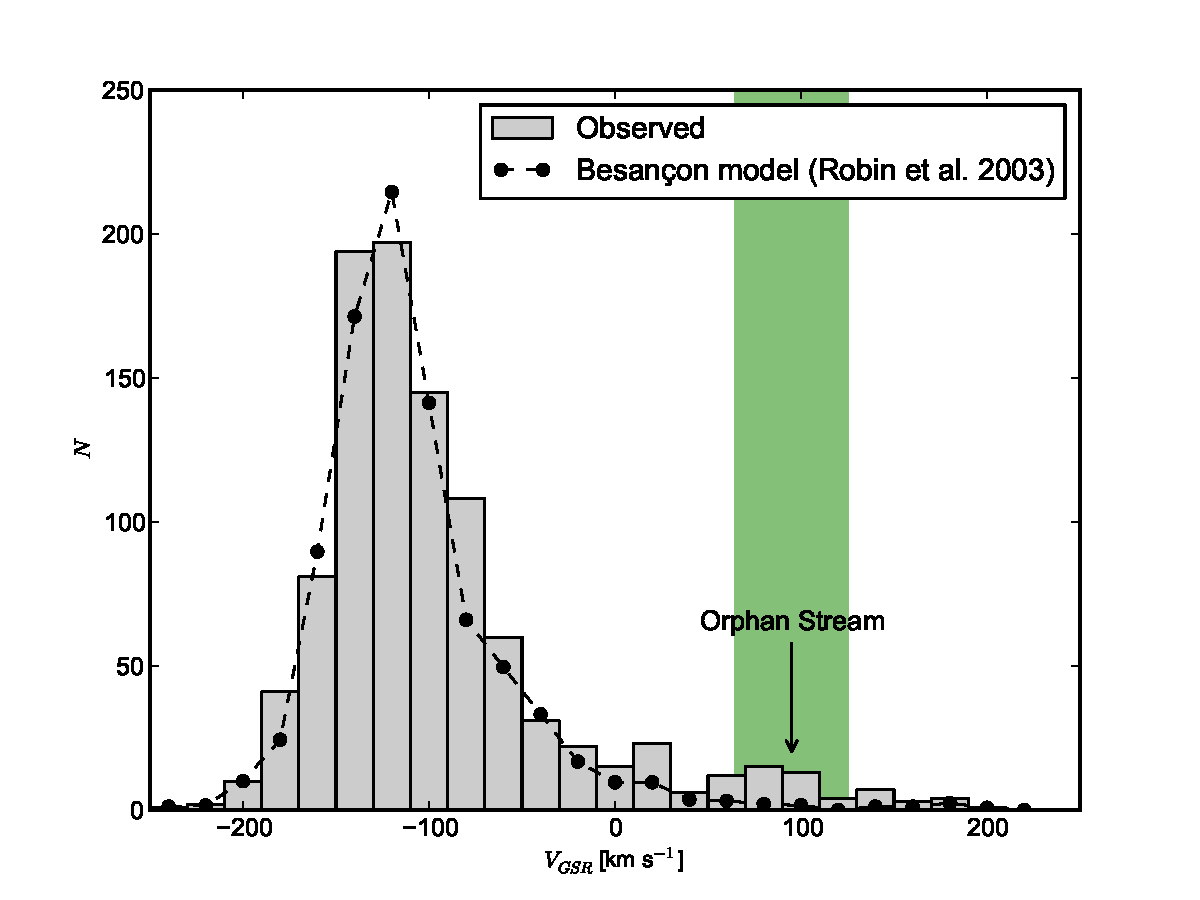
\includegraphics[width=\columnwidth]{./figures/vgsr-histogram.pdf}
	\caption{Galactocentric rest frame velocities for stars in both our observed fields (grey), and predicted Besan\c{c}on velocities which have been scaled to match our observed sample size. The expected kinematic signature from \citet{Newberg;et-al_2010} for the Orphan Stream is highlighted, as is our kinematic selection window (green).}
	\label{fig:velocities}
\end{figure}

In this region \citet{Newberg;et-al_2010} found the Orphan Stream to have $V_{\textsc{gsr}} = 110$ km s$^{-1}$ from BHB stars, approximately $105$\,km s$^{-1}$ on our scale. To isolate potential Orphan Stream members we have nominated a relatively wide kinematic selection region between $75 \leq V_{\textsc{gsr}} \leq 135$ km s$^{-1}$, which yields 25 Orphan Stream candidates. The typical uncertainty in our kinematics is $\pm{}3.5$\,km s$^{-1}$, although for our fainter targets this quickly increases to $\sim10$ km s$^{-1}$.

\subsection{Dwarf/Giant Discrimination}
\label{sec:dwarf-giant}

We have measured the equivalent widths of the gravity-sensitive Mg I line at 8807 \AA{} to distinguish dwarfs from giants \citep{Battaglia;Starkenburg_2012}. At a given temperature (or $g \-- r$) and metallicity, giant stars present narrow Mg I absorption lines than their dwarf contaminants. Given our target selection, our sample is likely to contain many more dwarfs than giants. In four cases no Mg I 8807 \AA{} line was apparent, so an upper limit was estimated based on the S/N. In these cases the candidate was considered a ``non-dwarf" because we cannot exclusively rule out a metal-poor sub-giant with this criterion alone. For these purposes we are only looking for a simple indication as to whether a star is likely a dwarf or not. Figure \ref{fig:ew-mg} illustrates the trend with EW$_{\lambda8807}$ against SDSS $g \-- r$ de-reddened\footnote{All magnitudes presented in this paper are de-reddened}, illustrating the dominant upper dwarf branch we wish to exclude. The adopted dwarf/giant separation line is shown. Admittedly this selection criterion is not particularly strict, but we are allowing multiple inclusive cuts and taking the intersection of these criteria to identify Orphan Stream giants.

\begin{figure}[h]
	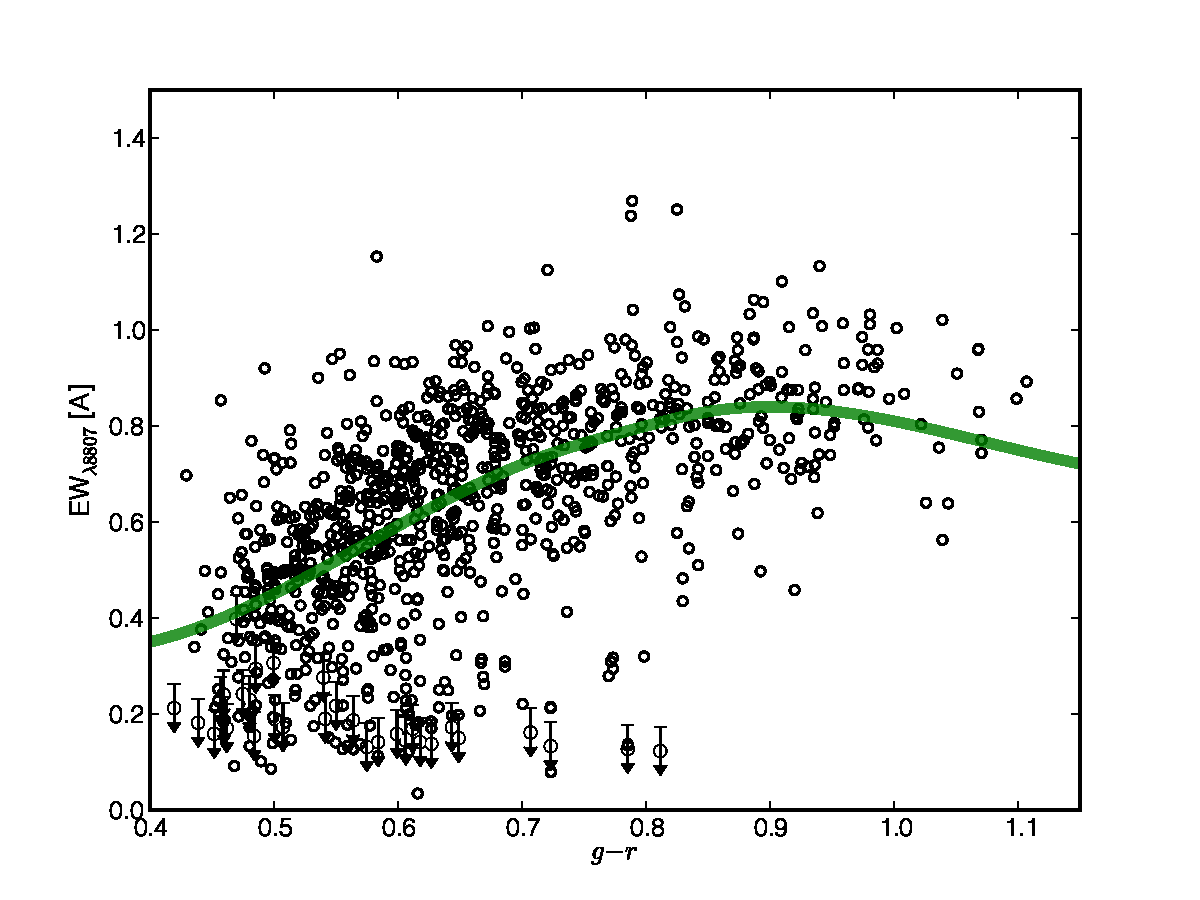
\includegraphics[width=\columnwidth]{./figures/ew-mg.pdf}
	\caption{De-reddened $g \-- r$ against the measured equivalent width of the Mg I transition at 8807 \AA{}. Dwarf contaminants occupy the more populous upper branch. Our separation line between dwarfs and giants is shown in green.}
	\label{fig:ew-mg}
\end{figure}

This analysis was also performed using the total equivalent width of the Mg\,\textsc{I}\,b triplet lines. Both analyses were entirely consistent with each other: essentially the same candidate selection was found using both techniques. However, given slightly poorer signal at the Mg\,\textsc{I}\,b triplet, we were forced to adopt many more upper limits than when using the 8807 {\AA} line. Because we classify all upper limits as being ``non-dwarfs" (i.e. potential OSS giants), we deduced a slightly larger candidate sample for the Mg\,\textsc{I}\,b analysis, which was primarily populated by upper limits. In conclusion, we found the Mg\,\textsc{I} line at 8807 appeared to be a more consistent dwarf discriminant given our weak S/N \--- particularly for our fainter stars \--- and thus we have used the 8807{\AA} Mg \textsc{I} selection throughout the rest of our analysis.

Our dwarf/giant separation line in Figure \ref{fig:ew-mg} yields 425 potential giants. This fraction of giants ($\sim{}44\%$) is much larger than what would be expected given our selection criterion (e.g. see \citet{Casey;et-al_2012a}). Hence, our gravity criterion is extremely inclusive and susceptible to dwarf contamination. Upon taking the intersection of our kinematic and gravity selections, we deduce eighteen stars that appear likely Orphan Stream K giants.


\subsection{Metallicities}
\label{sec:metallicities}

We have measured the equivalent widths of the Ca\,\textsc{II} near-infrared triplet lines for stars which meet our kinematic and surface gravity criteria. After correcting for luminosity, the equivalent width of the Ca\,\textsc{II} triplet lines provide a good indication for the metallicity of a RGB star \citep{Amandroff;Da_Costa_1991}. We have employed the \citet{Starkenburg;et-al_2010} relationship and corrected for luminosity in $g$ against the horizontal branch magnitude at $g_0$ = 17.1 \citep{Newberg;et-al_2010}. Strictly speaking, the Ca\,\textsc{II}\---[Fe/H] calibation is only valid for stars brighter than the horizontal branch, although the relationship only becomes significantly inappropriate near $g \-- g_{HB} \sim +1$ \citep{Saviane;et-al_2012}. Many of our candidates are fainter than this valid luminosity range, and therefore they should not be excluded solely because of their derived metallicities. Stars fainted than $g_0$ will have slightly lower metallicities than predicted by our Ca\,\textsc{II}\---[Fe/H] relationship, and for these stars we will only use metallicities to assign a relative qualitative likelihood for stream membership.

\begin{figure}[h]
	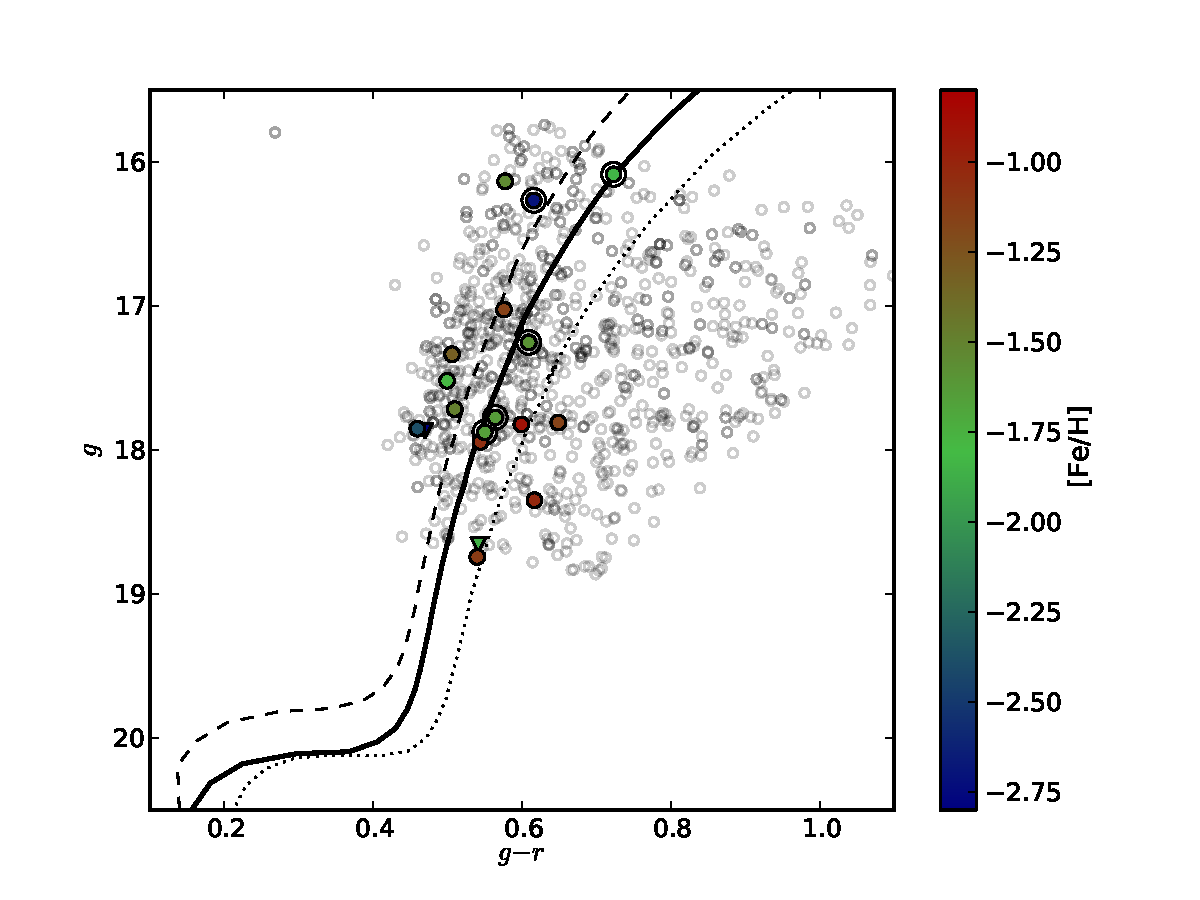
\includegraphics[width=\columnwidth]{./figures/cmd.pdf}
	\caption{Color magnitude diagram showing our observed candidates (grey) and highlighting candidates which meet our kinematic and gravity cuts. Candidates are colored by their metallicity, and those with upper limiting gravities are marked as triangles. Highly probable stream members are marked. Relevant 10 Gyr \citet{Girardi;et-al_2008} isochrones at $[\mbox{Fe/H}] = -1.5$ (dotted), $-2.0$ (dashed) at 21.4\,kpc \citep{Newberg;et-al_2010} are shown, as well as our best-fitting 10 Gyr isochrone of $[\mbox{Fe/H}] = -1.78$ at 24\,kpc (solid).}
	\label{fig:cmd}
\end{figure}

Figure \ref{fig:cmd} illustrates all eighteen candidates which meet both our kinematic and surface gravity criterion. Candidates are coloured by their metallicity deduced from the Ca\,\textsc{II} triplet. There are four candidates above $g_0 \sim 17.1$ which are within our valid luminosity range. One of these objects at $(g \-- r, g) \sim (0.57, 17)$ is +0.64\,dex more metal-rich than expected for the stream, and is excluded from membership. Another is only +0.21\,dex more metal-rich and sits at (0.57, 16.1), but it's position relative to the isochrone is inconsistent with our inferred metallicity. There appears to be an extremely metal-poor star in this sample with an estimated $[\mbox{Fe/H}] = -2.70$ which may be associated with the Orphan Stream. The likely parent system of the Orphan Stream is a Milky Way dwarf spheroidal \citep{Belokurov;et-al_2007, Sales;et-al_2008}, which are known to have a wide metallicity distribution function \citep{Tolstoy;et-al_2009}, including populations of extremely metal-poor stars \citep{Kirby;et-al_2010,Frebel;et-al_2010,Tafelmeyer;et-al_2010}. Thus, we keep this extremely metal-poor star as a potential stream member for follow-up chemical analysis. 
% speak about OSS 1?

\citet{Newberg;et-al_2010} found the median Orphan Stream metallicity to be [Fe/H] $= -2.1$ from BHB stars, and a distance of $21.4 \pm 1.0$\,kpc in this region. In Figure \ref{fig:cmd} we have overlaid 10 Gyr old isochrones from \citet{Girardi;et-al_2008} with metallicities of [Fe/H] $= -2.0$ and $-1.5$ at a distance of $21.4$ kpc \citep{Newberg;et-al_2010}. Four of our most probable Orphan Stream members fall between these isochrones. The brightest of these green points has an abundance which is in good agreement with the isochrone value. The line strength abundances for the other three stars (OSS 3, 6 and 7 \--- see Table \ref{tab:oss-members}) are less certain, as these stars are fainter than the horizontal branch. 

We can ascertain abundance corrections for our stars fainter than the horizontal branch by comparing our $g - g_{HB}$ (or $V-V_{HB}$) and $EW_{\lambda8452} + EW_{\lambda8662}$ with those measured by \citet{Saviane;et-al_2012} for globular clusters. Only two clusters from \citet{Saviane;et-al_2012} had measured Ca \textsc{II} equivalent widths for stars fainter than the horizontal branch: NGC 6397 with $[\mbox{Fe/H}] = -1.99$ and NGC 6254 with $[\mbox{Fe/H}] = -1.57$ \citep[both abundances from][]{Carretta;et-al_2009}. OSS 6 and OSS 7 lie at the mid-point between these cluster stars, implying an abundance of $[\mbox{Fe/H}] \sim -1.78$, or a mean correction of $-0.14$ dex for OSS 6 and 7. Although OSS 3 is 0.15 magnitudes fainter than the horizontal branch, it has equivalent widths consistent with our inferred metallicity of $[\mbox{Fe/H}] = -1.62$, so no correction was made. With corrections included for OSS 6 and 7 we find a median stream metallicity from our four most probable stars of $[\mbox{Fe/H}] = -1.78 \pm 0.08$, which is slightly more metal-rich than the $[\mbox{Fe/H}] =-2.1$ found by \citet{Newberg;et-al_2010} from BHB stars. If we include our EMP candidate, the median decreases by 0.01 dex and the spread increases to 0.39\,dex. 

Given that our four Orphan Stream stars cover range along the giant branch, we are in a good position to revise the distance estimate to the stream. Given a 10 Gyr \citet{Girardi;et-al_2008} isochrone at $[\mbox{Fe/H}] = -1.74$, we find a best-fitting distance to the stream of 24 kpc at ($l, $b) = ($250^\circ$, $50^\circ$). This isochrone is also shown in Figure \ref{fig:cmd}, and it is clear that the four most probable member stars lie almost precisely on this isochrone. Our derived distance is slightly farther than the $21.4 \pm 1.0$ kpc found by \citet{Newberg;et-al_2010}, but given the inherent uncertainties in determining distance we argue these distances are largely in agreement.




\begin{deluxetable*}{lcccccccccl}
\tabletypesize{\scriptsize}
\tablecaption{Identified Orphan Stream Members\label{tab:oss-members}}
\tablehead{
	\colhead{Star} &
	\colhead{$\alpha$} &
	\colhead{$\delta$} &
	\colhead{$g$} &
	\colhead{$g \-- r$} &
	\colhead{$V_{helio}$} &
	\colhead{$V_{\textsc{gsr}}$} &
	\colhead{$V_{err}$} &
	\colhead{$EW_{\lambda8807}$} &
	\colhead{[Fe/H]} &
	\colhead{Comment} \\
Name & (J2000) & (J2000) & & & (kms $^{-1}$) & (km s$^{-1}$) & (km s$^{-1}$) & (\AA) & (dex)
}
\startdata
OSS 1 & 10 46 50.6 & $-$00 13 17.9 & 17.33 & 0.50  &  215.5  & 77.0 & 4.0 & 0.416 & $-1.31$ & Unlikely member! \\
OSS 2 & 10 47 17.6 & $+$00 25 07.7 & 16.09 &  0.73 &  215.7  & 79.2 & 3.3 & 0.212 & $-1.84$ & Highly probable member \\
OSS 3 & 10 47 30.1 & $-$00 01 24.6 & 17.25 &  0.61 &  221.4  & 83.6 & 3.4 & 0.123 & $-1.62$ & Highly probable member \\
OSS 4 & 10 49 08.3 & $+$00 02 00.2 & 16.27 &  0.62 &  218.5  & 81.5 & 4.6 & 0.034 & $-2.70$ & Possible EMP member \\
OSS 6 & 10 48 20.9 & $+$00 26 34.4 & 17.88 &  0.55 &  254.9  & 118.8 & 11.7 & 0.469 & $-1.79$\tablenotemark{a} & Highly probable member \\
OSS 7 & 10 46 29.3 & $-$00 19 38.5 & 17.77 &  0.56 &  217.3  & 78.4 & 5.2 & 0.126 & $-1.77$\tablenotemark{a} & Highly probable member 
\enddata
\tablenotetext{a}{Abundance correction of $-0.14$\,dex included (see \S\ref{sec:metallicities}).}
\end{deluxetable*}

\section{Conclusion}
\label{sec:conclusions}

We have presented a detailed analysis to isolate individual Orphan Stream K giants from low resolution spectroscopy using a combination of photometric, kinematic, gravity, and metallicity information. Although each individual criterion is likely to induce some level contamination, their intersection reveals highly probable, self-consistent, Orphan Stream K giants.  We deduce a stream metallicity of $[\mbox{Fe/H}] = -1.78 \pm 0.08$ which is not biased by spectral type. Recall that the metallicity determination was performed after kinematic and gravity cuts, and our most probable members lay perfectly on a 10 Gyr isochrone of $[\mbox{Fe/H}] = -1.78$. Our stream members indicate a revised distance to the stream of $24$\,kpc at $(l, b) = (250\,^\circ$, $50\,^\circ)$, slightly farther than that deduced by \citet{Newberg;et-al_2010}.

If the Orphan Stream continues through SEGUE stripe 1540 at $(l, b) = (271\,^\circ$, $38\,^\circ)$ as \citet{Newberg;et-al_2010} found, then the stream is even closer there than in the region analysed here. Thus, if our observations and analyses are repeated at $(271\,^\circ$, $38\,^\circ)$, we predict K giant stream members of brighter apparent magnitude will be recovered. If the stream density is similar to or higher than what we observe at $(l, b) = (250\,^\circ, 50\,^\circ)$ then more K giant Orphan Stream members are likely to be recovered in the stripe 1540 field.

Although OSS 6 has an uncertain radial velocity, using a maximum-likelihood estimation we find the mean stream galactocentric velocity at $(l, b) = (250\,^\circ, 50\,^\circ)$ from five stars to be $V_{GSR} = 82 \pm 1.6$ km s$^{-1}$ and the intrinsic dispersion to be $0.3 \pm 3.3$ km s$^{-1}$. For our four stars with low radial velocity errors this dispersion is found to be $0.00 \pm 2.4$ km s$^{-1}$. These velocities indicate that the Orphan Stream is a very cold stream, and implies their motion is largely perpendicular to the line of sight.

The K giants presented here can provide great insight into the chemistry, and history of the Orphan Stream. High resolution spectroscopic observations have been taken for our most highly probable members and a detailed chemical analysis will be presented in a forthcoming paper (Casey et al. 2012c, in preparation). Detailed chemical abundances can help determine both the nature of the host system, and allow us to compare peculiar chemical signatures with those of the known Milky Way satellites in order to associate likely parents. However at least for the moment, the Orphan Stream remains appropriately named.


\acknowledgements
ARC acknowledges the financial support through the Australian Research Council Laureate Fellowship 0992131, and from the Australian Prime Minister's Endeavour Award Research Fellowship, which has facilitated his research at MIT. SK and GDaC acknowledge the financial support from the Australian Research Council through Discovery Programs DP0878137 and DP120101237.

Funding for the SDSS and SDSS-II has been provided by the Alfred P. Sloan Foundation, the Participating Institutions, the National Science Foundation, the U.S. Department of Energy, the National Aeronautics and Space Administration, the Japanese Monbukagakusho, the Max Planck Society, and the Higher Education Funding Council for England. The SDSS Web Site is http://www.sdss.org/.

The SDSS is managed by the Astrophysical Research Consortium for the Participating Institutions. The Participating Institutions are the American Museum of Natural History, Astrophysical Institute Potsdam, University of Basel, University of Cambridge, Case Western Reserve University, University of Chicago, Drexel University, Fermilab, the Institute for Advanced Study, the Japan Participation Group, Johns Hopkins University, the Joint Institute for Nuclear Astrophysics, the Kavli Institute for Particle Astrophysics and Cosmology, the Korean Scientist Group, the Chinese Academy of Sciences (LAMOST), Los Alamos National Laboratory, the Max-Planck-Institute for Astronomy (MPIA), the Max-Planck-Institute for Astrophysics (MPA), New Mexico State University, Ohio State University, University of Pittsburgh, University of Portsmouth, Princeton University, the United States Naval Observatory, and the University of Washington.

\bibliographystyle{apj}
\bibliography{bibliography}
\end{document}
